% Preambulo compartido para clases en formato beamer
\documentclass[9pt, xcolor=svgnames]{beamer}
\usepackage[utf8]{inputenc}
\usepackage[T1]{fontenc}
\usepackage[spanish,es-nodecimaldot]{babel}

\usetheme[progressbar=frametitle]{metropolis}
\metroset{sectionpage=none, subsectionpage=none}
\usepackage{appendixnumberbeamer}
\usepackage{booktabs}
\usepackage{amsmath,amssymb,bm,mathtools}
\usepackage{physics}
\usepackage{graphicx}
\usepackage{multicol}
\usepackage{tikz}
\usepackage{minted}
\usemintedstyle{tango}
\setminted{fontsize=\scriptsize, breaklines=true, linenos=true, bgcolor=LightGray!20, frame=lines}
\newminted{python}{fontsize=\scriptsize, breaklines=true, linenos=true, bgcolor=LightGray!20, frame=lines}
\usepackage{pgfplots}
\pgfplotsset{compat=1.18}
\usepackage{ragged2e}
\usepackage{xspace}
\newcommand{\themename}{\textbf{\textsc{metropolis}}\xspace}

\setbeamercolor{block title}{bg=MidnightBlue!85, fg=white}
\setbeamercolor{block body}{bg=MidnightBlue!5, fg=black}
\setbeamercolor{alerted text}{fg=Crimson}
\setbeamercolor{frametitle}{bg=MidnightBlue!10, fg=black}
\setbeamertemplate{blocks}[rounded][shadow=true]


\title[Modelos Computacionales]{Modelos Computacionales CFIS261}

\author[Joaquín Peralta]{\Large{Joaquín Peralta\texttt{<joa.peralta@uandresbello.edu>}}}
\titlegraphic{\hfill
\includegraphics[height=2cm]{logo-unab.jpg}}

\date{Sesion 01}

\begin{document}

\frame{\titlepage}

%------------------------------------------------

\begin{frame}
\frametitle{Clase 1: Mapas no lineales}

En esta sesión introduciremos uno de los sistemas dinámicos más
importantes en dinámica no lineal.

\begin{block}{Objetivos}
\begin{itemize}
\item Repaso de gráficos con \texttt{matplotlib}
\item Modelar crecimiento de poblaciones
\item Introducir el \textbf{mapa logístico}
\item Comprender \textbf{puntos fijos}
\item Introducir \textbf{atractores}
\item Entender el origen del \textbf{caos determinista}
\item Construir el \textbf{diagrama de bifurcación}
\end{itemize}
\end{block}

\end{frame}

%------------------------------------------------

\begin{frame}
\frametitle{Gráficos de líneas}

Un gráfico de línea representa una función

\[
y=f(x)
\]

evaluada en muchos puntos.

\begin{center}
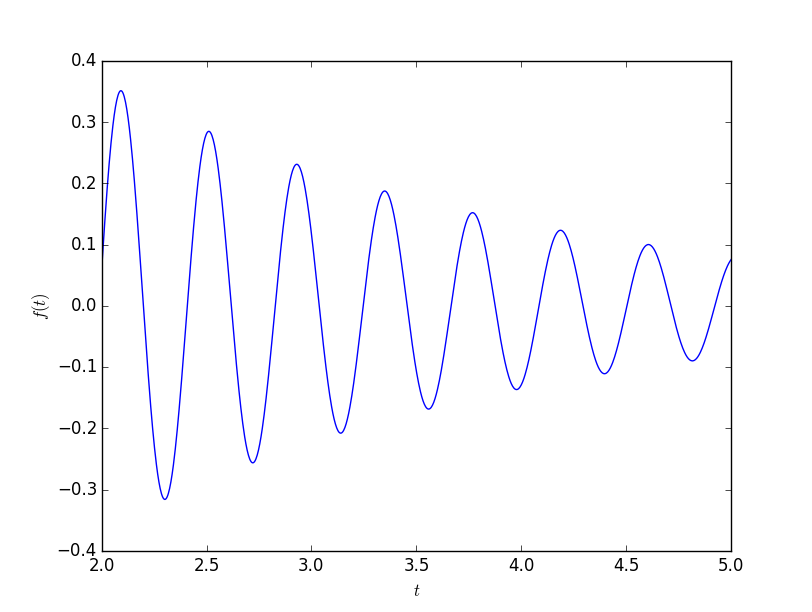
\includegraphics[scale=0.2]{plot.png}
\end{center}

Aplicaciones comunes:

\begin{itemize}
\item evolución temporal
\item funciones matemáticas
\item resultados de simulaciones
\end{itemize}

\end{frame}

%------------------------------------------------

\begin{frame}[fragile]
\frametitle{Gráficos de líneas (código)}

\begin{pythoncode}
from math import *
import matplotlib.pyplot as plt
import numpy as np

def f(t):
    return exp(-t/2.0)*cos(15.0*t)

X = np.linspace(2.0,5.0,1000)
Y = [f(x) for x in X]

plt.plot(X,Y,'b-')
plt.xlabel("$t$")
plt.ylabel("$f(t)$")
plt.show()
\end{pythoncode}

\end{frame}

%------------------------------------------------

\begin{frame}
\frametitle{Gráficos de dispersión}

Un gráfico de dispersión representa pares de datos

\[
(x_i,y_i)
\]

sin conectar los puntos.

\begin{center}
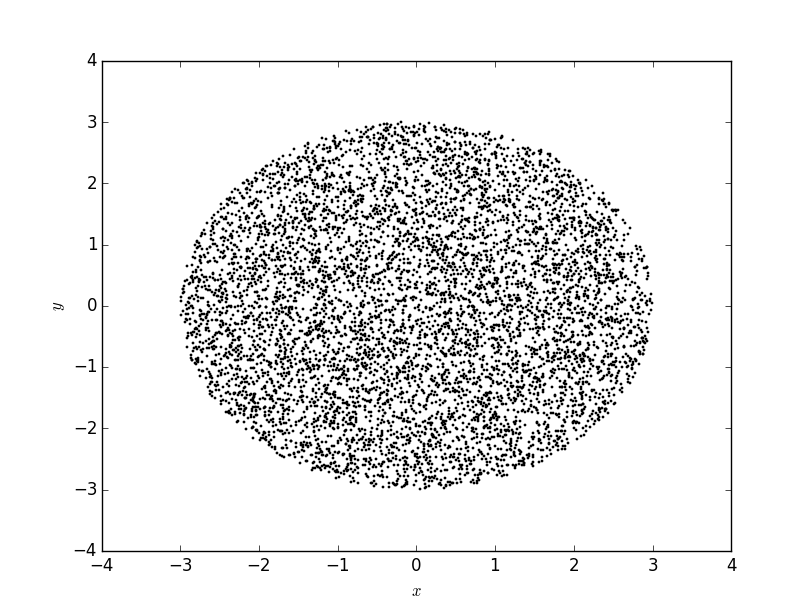
\includegraphics[scale=0.2]{scatter.png}
\end{center}

Se usa frecuentemente en

\begin{itemize}
\item simulaciones Monte Carlo
\item datos experimentales
\item distribuciones espaciales
\end{itemize}

\end{frame}

%------------------------------------------------

\begin{frame}
\frametitle{Histogramas}

Un histograma permite estimar la distribución de probabilidad
de una variable aleatoria.

\begin{center}
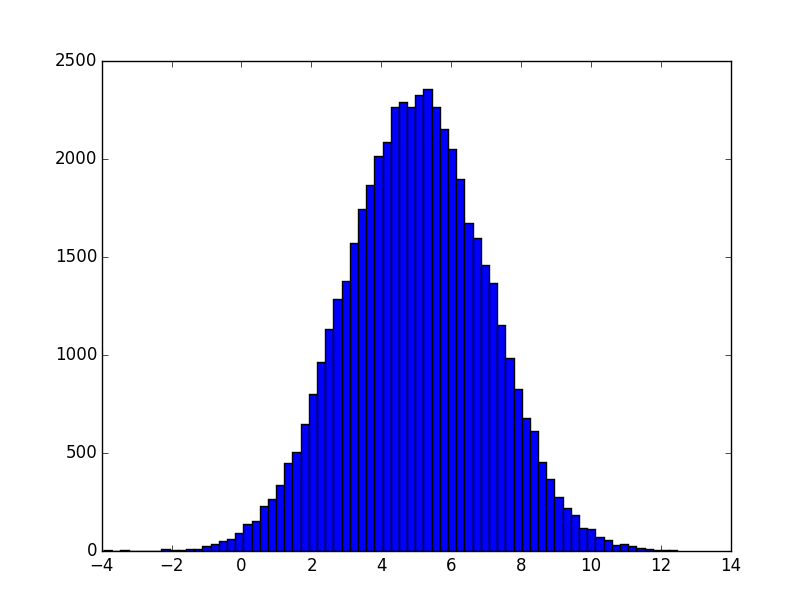
\includegraphics[scale=0.2]{histogram.png}
\end{center}

Procedimiento:

\begin{enumerate}
\item generar datos
\item dividir el eje en intervalos
\item contar frecuencia de cada intervalo
\end{enumerate}

\end{frame}

%------------------------------------------------

\begin{frame}
\frametitle{Crecimiento de poblaciones}

Supongamos que una población $N(t)$ crece proporcionalmente
a su tamaño actual.

\[
\frac{dN}{dt}=\lambda N
\]

La solución es

\[
N(t)=N(0)e^{\lambda t}
\]

\begin{block}{Problema}
Para $\lambda>0$ la población crece indefinidamente.
Esto no es realista debido a recursos limitados.
\end{block}

\end{frame}

%------------------------------------------------

\begin{frame}
\frametitle{Modelo logístico}

Introducimos una población máxima $N^*$.

\[
\frac{dN}{dt}=\lambda'(N^*-N)N
\]

Interpretación:

\begin{itemize}
\item si $N\ll N^*$ crecimiento casi exponencial
\item si $N\approx N^*$ crecimiento disminuye
\item si $N>N^*$ población decrece
\end{itemize}

Este es un modelo \textbf{no lineal}.

\end{frame}

%------------------------------------------------

\begin{frame}
\frametitle{Discretización}

Aproximamos la derivada

\[
\frac{dN}{dt}\approx
\frac{N(t+\Delta t)-N(t)}{\Delta t}
\]

Entonces

\[
N(t+\Delta t)=N(t)+\lambda'\Delta t(N^*-N(t))N(t)
\]

Definimos

\[
N_i=N(t)
\qquad
N_{i+1}=N(t+\Delta t)
\]

\[
N_{i+1}=N_i+\lambda'\Delta t(N^*-N_i)N_i
\]

\end{frame}

%------------------------------------------------

\begin{frame}
\frametitle{Mapa logístico}

Definimos

\[
x_i=\frac{N_i}{N^*}
\]

y

\[
\mu=1+\lambda'\Delta t N^*
\]

Obtenemos

\begin{block}{Mapa logístico}

\[
x_{i+1}=\mu x_i(1-x_i)
\]

\end{block}

Este mapa simple produce dinámica muy compleja.

\end{frame}

%------------------------------------------------

\begin{frame}
\frametitle{Puntos fijos}

Un punto fijo satisface

\[
f(x_0)=x_0
\]

Para el mapa logístico

\[
x_{i+1}=\mu x_i(1-x_i)
\]

tenemos dos puntos fijos:

\[
x_0=0
\]

\[
x_0=\frac{\mu-1}{\mu}
\]

\end{frame}

%------------------------------------------------

\begin{frame}
\footnotesize
\frametitle{Estabilidad de un punto fijo}

Sea un mapa iterativo

\[
x_{n+1}=f(x_n)
\]

Un punto fijo satisface

\[
f(x_0)=x_0
\]

Para estudiar su estabilidad, perturbamos ligeramente el sistema:

\[
x_n = x_0 + \epsilon_n
\]

donde $\epsilon_n$ es una perturbación pequeña.

\vspace{4mm}

La evolución es

\[
x_{n+1}=f(x_0+\epsilon_n)
\]

Expandiendo en serie de Taylor alrededor de $x_0$:

\[
f(x_0+\epsilon_n)
\approx
f(x_0)+f'(x_0)\epsilon_n
\]

Como $f(x_0)=x_0$, obtenemos

\[
x_{n+1}=x_0+f'(x_0)\epsilon_n
\]

\end{frame}



\begin{frame}
\frametitle{Condición de estabilidad}

Restando $x_0$ en ambos lados:

\[
\epsilon_{n+1}=f'(x_0)\epsilon_n
\]

Luego

\[
\epsilon_n = (f'(x_0))^n \epsilon_0
\]

Esto implica:

\begin{itemize}
\item Si $|f'(x_0)|<1$ las perturbaciones disminuyen
\item Si $|f'(x_0)|>1$ las perturbaciones crecen
\end{itemize}

\begin{block}{Condición de estabilidad}

\[
|f'(x_0)| < 1
\]

\end{block}

En ese caso el punto fijo es un \textbf{atractor}.

\end{frame}



\begin{frame}
\frametitle{Estabilidad del mapa logístico}

El mapa logístico es

\[
x_{n+1}=\mu x_n(1-x_n)
\]

La derivada es

\[
f'(x)=\mu(1-2x)
\]

Uno de los puntos fijos es

\[
x_0=\frac{\mu-1}{\mu}
\]

Evaluando la derivada:

\[
f'(x_0)=\mu\left(1-2\frac{\mu-1}{\mu}\right)
\]

\[
f'(x_0)=\mu(1-2+2/\mu)
\]

\[
f'(x_0)=2-\mu
\]

\end{frame}


\begin{frame}
\footnotesize
\frametitle{Condición de estabilidad}

Recordemos que la condición es

\[
|f'(x_0)|<1
\]

Como

\[
f'(x_0)=2-\mu
\]

entonces

\[
|2-\mu|<1
\]

Esto implica

\[
1<\mu<3
\]

\begin{block}{Resultado}

Para

\[
\mu<3
\]

el punto fijo es estable.

Para

\[
\mu>3
\]

aparecen oscilaciones de período 2.

\end{block}

\end{frame}

%------------------------------------------------

\begin{frame}
\frametitle{Cobweb diagram}

Para visualizar iteraciones del mapa se usa
un \textbf{diagrama de telaraña}.

Procedimiento:

\begin{enumerate}
\item graficar $y=f(x)$
\item graficar $y=x$
\item iterar gráficamente
\end{enumerate}

Esto permite observar

\begin{itemize}
\item convergencia
\item ciclos
\item caos
\end{itemize}

\end{frame}

%------------------------------------------------

\begin{frame}[fragile]
\frametitle{Cobweb (código Python)}

\begin{pythoncode}
import numpy as np
import matplotlib.pyplot as plt

mu = 3.2

def f(x):
    return mu*x*(1-x)

x = np.linspace(0,1,500)

plt.plot(x,f(x))
plt.plot(x,x)

xn = 0.2

for i in range(50):

    xnext = f(xn)

    plt.plot([xn,xn],[xn,xnext],'r')
    plt.plot([xn,xnext],[xnext,xnext],'r')

    xn = xnext

plt.show()
\end{pythoncode}

\end{frame}

%------------------------------------------------

\begin{frame}
\frametitle{Atractores}

Un atractor es un estado hacia el cual
evolucionan muchas condiciones iniciales.

Dependiendo de $\mu$ podemos tener

\begin{itemize}
\item punto fijo
\item ciclo de período 2
\item ciclo de período 4
\item caos
\end{itemize}

\end{frame}

%------------------------------------------------

\begin{frame}
\frametitle{Ejemplos}

\begin{center}
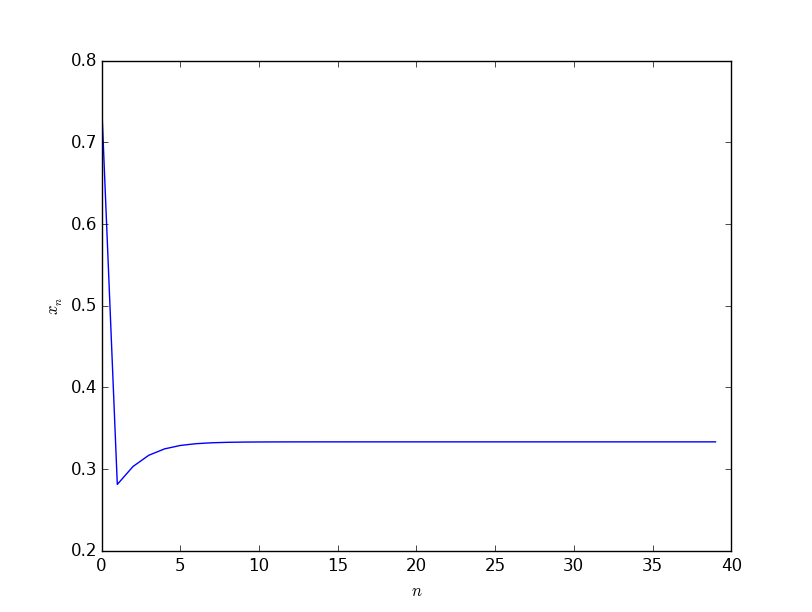
\includegraphics[scale=0.45]{Convergence1.png}
\end{center}

\end{frame}

%------------------------------------------------

\begin{frame}
\frametitle{Doblamiento de período}

Al aumentar $\mu$ ocurre

\begin{itemize}
\item punto fijo
\item período 2
\item período 4
\item período 8
\item caos
\end{itemize}

Este mecanismo se llama

\textbf{doblamiento de período}.

\end{frame}

%------------------------------------------------

\begin{frame}
\frametitle{Diagrama de bifurcación}

\begin{center}
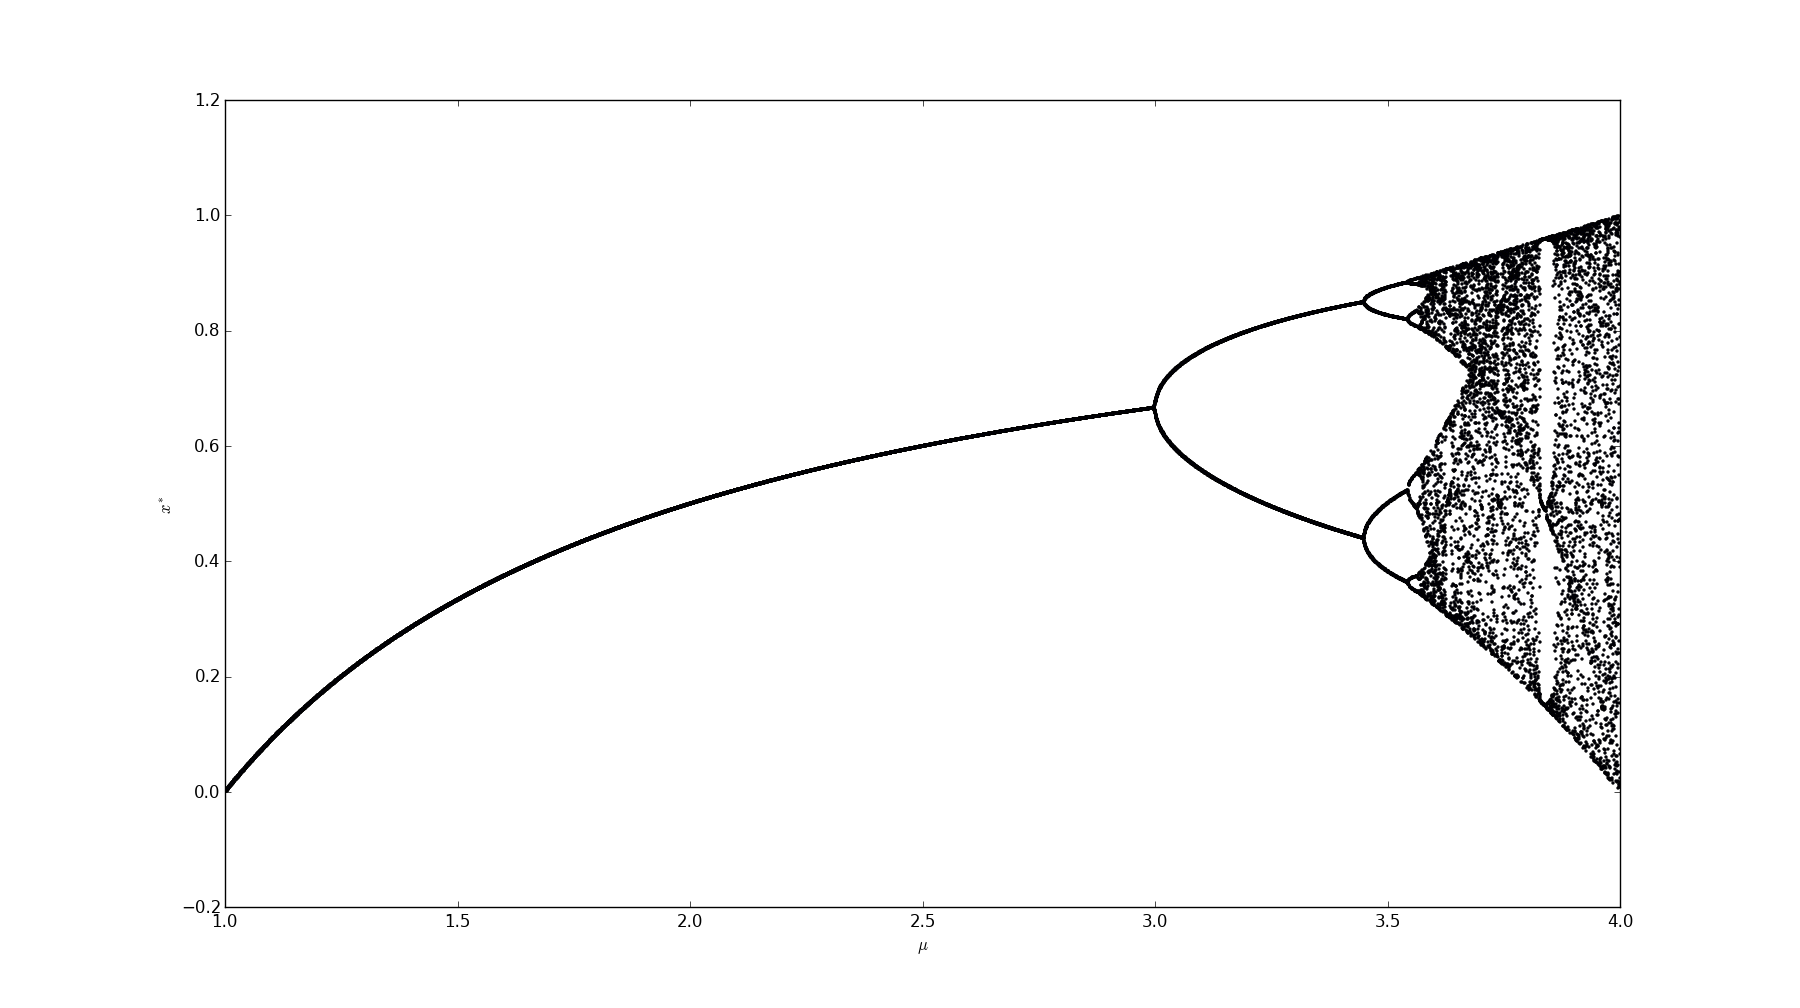
\includegraphics[scale=0.26]{Bifurcation.png}
\end{center}

Cada punto representa un estado estable
para un valor de $\mu$.

\end{frame}

%------------------------------------------------

\begin{frame}[fragile]
\frametitle{Bifurcation diagram (código)}

\begin{pythoncode}
import numpy as np
import matplotlib.pyplot as plt

n = 1000
mu_values = np.linspace(2.5,4,n)

iterations = 1000
last = 100

for mu in mu_values:

    x = 0.5

    for i in range(iterations):
        x = mu*x*(1-x)

        if i >= iterations-last:
            plt.plot(mu,x,'k.',markersize=1)

plt.xlabel("$\mu$")
plt.ylabel("$x$")
plt.show()
\end{pythoncode}

\end{frame}

%------------------------------------------------

\begin{frame}
\frametitle{Exponente de Lyapunov}

Mide la sensibilidad a condiciones iniciales.

\[
\lambda =
\lim_{n\to\infty}
\frac{1}{n}
\sum_{i=0}^{n-1}
\ln |f'(x_i)|
\]

Interpretación:

\begin{itemize}
\item $\lambda<0$ sistema estable
\item $\lambda=0$ transición
\item $\lambda>0$ caos
\end{itemize}

\end{frame}

%------------------------------------------------

\begin{frame}
\frametitle{Actividades}

\begin{enumerate}

\item Simule el mapa logístico para

\[
\mu=2.6,3.1,3.7,3.8,3.9,3.99
\]

\item Construya el diagrama de bifurcación.

\item Para $\mu=3.99$ genere $100000$ iteraciones
y calcule el histograma de $x$.

\end{enumerate}

\end{frame}

\end{document}